% Optimisation optique physique et aérodynamique
\chapter{Optimisation Bidisciplinaire : Optique Physique et CFD}
\nomenclature[S]{CFD}{Dynamique des fluides numérique (Computational Fluid Dynamics)}
\chaptermark{Optim OP-CFD}
\section[Présentation du cas de référence]{Présentation du cas de référence\sectionmark{Cas de référence}}
\sectionmark{Cas de référence}
\nomenclature[S]{GFA}{Géométrie de référence (Generic Fighter Aircraft)}%

\lipsum
\subsection{Géométrie}
\lipsum

\begin{figure}[htp]
    \centering
    
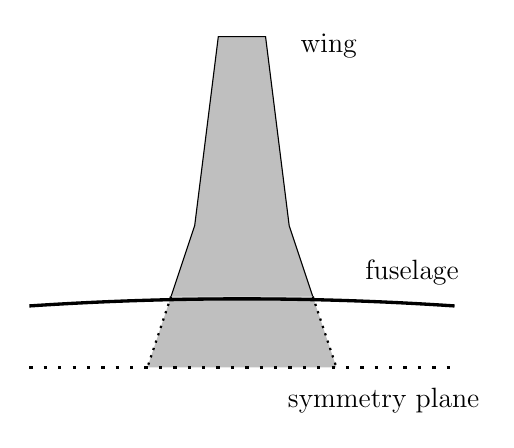
\begin{tikzpicture}[scale=0.6,every node/.style={scale=0.7}]
    \node[anchor=west] at (1.1,6.8){\Large wing};
    \node[anchor=south] at (3.6,1.6) {\Large fuselage};
    \node[anchor=north] at (3,-0.3) {\Large symmetry plane};

    \draw[fill=lightgray] (1.5,1.5) -- (1,3) -- (0.5,7) -- (-0.5,7) -- (-1,3) -- (-1.5,1.5);

    \draw[draw=none,fill=lightgray] (-1.5,1.5) -- (-2,0) -- (2,0) -- (1.5,1.5);
    \draw[thick,dotted] (-1.5,1.5) -- (-2,0);
    \draw[thick,dotted] (1.5,1.5) -- (2,0);

    \draw[very thick] (-4.5,1.3) .. controls (-1.5,1.5) and (1.5,1.5) .. (4.5,1.3);

    \node at (0,2.5){\Huge \sref};

    \draw[very thick,loosely dotted] (-4.5,0) -- (4.5,0);
\end{tikzpicture}

    \caption{Définition de la \sref{}.}
    \label{fig:sref}
\end{figure}

\subsection{Analyse aérodynamique}
\lipsum
\subsection{Analyse SER}
\nomenclature[S]{SER}{Surface \'Equivalente radar}

\lipsum
\section[Présentation des outils d'optimisation]{Présentation des outils d'optimisation\sectionmark{Outils}}
\sectionmark{Outils}
\lipsum
\subsection{Présentation du processus d'optimsation}
\lipsum

\begin{figure}[htp]
    \centering
    \begin{tikzpicture}[node distance=\nd,scale=0.7,every node/.style={transform shape}]
    \tikzstyle{startstop} = [rectangle,rounded corners, minimum width=.5\ndv, minimum height=.5\nd,text centered,draw=black,fill=red!30]

    \tikzstyle{io} = [trapezium, trapezium left angle=70, trapezium right angle=110, minimum width=.5\ndv,  minimum height=.5\nd,  text centered, draw=black, fill=blue!20,execute at begin node={\begin{varwidth}{\ndv}\centering},execute at end node={\end{varwidth}}]

    \tikzstyle{process} = [rectangle, minimum width=.5\ndv,  minimum height=.5\nd, text centered, draw=black, fill=orange!30,execute at begin node={\begin{varwidth}{\ndv}\centering},execute at end node={\end{varwidth}}]

    \tikzstyle{decision} = [diamond, minimum width=.5\ndv, minimum height=.5\nd,aspect=2,  text centered,   draw=black, fill=green!30,execute at begin node={\begin{varwidth}{\ndv}\centering},execute at end node={\end{varwidth}}]

    \tikzstyle{dummy} = [rectangle,draw=none,fill=none,minimum height=.5\nd,minimum width=.5\ndv]

    \tikzstyle{line} = [thick]

    \tikzstyle{arrow} = [line,->,>=stealth]


    \node (start) [startstop] {Start};
    \node (init) [io,below of=start] {Initial state};
    \node (optim) [process, below of=init] {Optimizer};
    \node (cvg) [decision, below of=optim,yshift=-.5\nd]{convergence};
    \node (DV) [io,below of=cvg,yshift=-.5\nd] {Design Variable};
    \node (cad) [process,below of=DV] {CAD modeler};
    \node (in2d) [io,left of=cad,xshift=-1.5\ndv]{Initial geometry\newline Initial 2D grids};
    \coordinate [below of=cad,yshift=.5\nd] (aux0);

    \node (POgrid) [io,below of=cad,xshift=.5\ndv] {PO 2D grid};
    \node (COPOLA) [process,below of=POgrid,yshift=-2\nd] {COPOLA code};
    \node (RCS) [io,below of=COPOLA,yshift=-.5\nd] {RCS};
    \node (dRCS) [io,right of=RCS,xshift=.5\ndv] {%
    RCS\newline gradient};

    \node (CFDgrid) [io,below of=cad,xshift=-.5\ndv] {CFD 2D grid};
    \node (3Ddef) [process,below of=CFDgrid] {elliptic operator};
    \node (in3d) [io,left of=3Ddef,xshift=-\ndv] {Initial 3D mesh};
    \node (Vmesh)[io,below of=3Ddef] {3D mesh};
    \node (aether) [process,below of=Vmesh] {CFD code};
    \node (aerovar) [io,below of=aether,yshift=-.5\nd] {\cd,\cl};

    \node (aetherlin) [process,left of=aether,xshift=-.5\ndv] {CFD adjoint solver};
    \node (aerograd) [io,below of=aetherlin,yshift=-.5\nd]{Aerodynamic gradient};

    \node (costgather) [process,below of=cad,yshift=-6.5\nd] {Cost Gather};

    \coordinate[above of=costgather] (aux);

    \node (obs) [io,right of=optim,xshift=1\ndv] {Cost, constraints, gradients};

    \node (end) [startstop,left of=cvg,xshift=-1.5\ndv] {Stop};

    \draw[arrow] (start) -- (init);
    \draw[arrow] (init) -- (optim);
    \draw[arrow] (optim) -- (cvg);
    \draw [arrow] (cvg) -- node[anchor=east] {no} (DV);
    \draw[arrow] (DV) -- (cad);
    \draw[line] (cad) -- (aux0);
    \draw[arrow] (aux0) -| (POgrid);
    \draw[arrow] (POgrid) -- (COPOLA);
    \draw[arrow] (COPOLA) -- (RCS);
    \draw[arrow] (COPOLA) -| (dRCS);

    \draw[arrow] (in2d) -- (cad);
    \draw[arrow] (in3d) -- (3Ddef);

    \draw[arrow] (aux0) -| (CFDgrid);
    \draw[arrow] (CFDgrid) -- (3Ddef);
    \draw[arrow] (3Ddef) -- (Vmesh);
    \draw[arrow] (Vmesh) -- (aether);
    \draw[arrow] (aether) -- (aerovar);

    \draw[arrow] (aether) -- (aetherlin);
    \draw[arrow] (aetherlin) -- (aerograd);

    \draw[line] (RCS) |- (aux) ;
    \draw[line] (dRCS) |- ($(RCS)-(0,\nd)$) ;
    \draw[line] (aerovar) |- (aux) ;
    \draw[line] (aerograd) |- ($(aerovar)-(0,\nd)$) ;
    \draw[arrow] (aux) -- (costgather);

    \draw [arrow] (costgather) -- ++ (2.1\ndv,0) |- (obs);
    \draw [arrow] (obs) -- (optim);

    \draw [arrow] (cvg) -- node[anchor=south] {yes} (end);
\end{tikzpicture}

    \caption{Organigrame du processus d'optimisation automatique.}
    \label{fig:optim-process}
\end{figure}

\subsection{Présentation du modeleur CAO}
\nomenclature[S]{CAO}{Conception Assistée par Ordinateur}
\nomenclature[C]{GANIMEDE}{Modeleur CAO}
\lipsum

\section{Coûts et Contraintes}
\lipsum

\begin{figure}
	\centering
    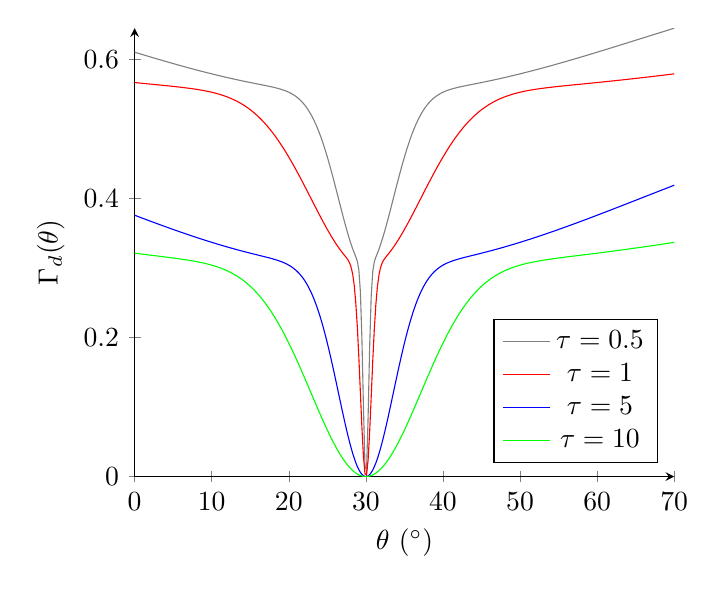
\begin{tikzpicture}
\begin{axis}
		[
			axis lines = left,
			xlabel = $\theta\ (^\circ)$,
			ylabel = {$\Gamma_d(\theta)$},
			legend pos = south east,
		]
	\addplot
		[
			domain = 0:70,
			samples = 350,
			color = gray,
		]
	{1 - 1/2*(
		((6-0)/10)*exp(-((x-30)/(0.5*10^0))^2) +
		((6-1)/10)*exp(-((x-30)/(0.5*10^1))^2) +
		((6-2)/10)*exp(-((x-30)/(0.5*10^2))^2) +
		((6-3)/10)*exp(-((x-30)/(0.5*10^3))^2) +
		((6-4)/10)*exp(-((x-30)/(0.5*10^4))^2) )
	};
	\addlegendentry{$\tau = 0.5$}
	\addplot
		[
			domain = 0:70,
			samples = 350,
			color = red,
		]
	{1 - 1/2*(
		((6-0)/10)*exp(-((x-30)/(1*10^0))^2) +
		((6-1)/10)*exp(-((x-30)/(1*10^1))^2) +
		((6-2)/10)*exp(-((x-30)/(1*10^2))^2) +
		((6-3)/10)*exp(-((x-30)/(1*10^3))^2) +
		((6-4)/10)*exp(-((x-30)/(1*10^4))^2) )
	};
	\addlegendentry{$\tau = 1$}
	\addplot
		[
			domain = 0:70,
			samples = 350,
			color = blue,
		]
	{1 - 1/2*(
		((6-0)/10)*exp(-((x-30)/(5*10^0))^2) +
		((6-1)/10)*exp(-((x-30)/(5*10^1))^2) +
		((6-2)/10)*exp(-((x-30)/(5*10^2))^2) +
		((6-3)/10)*exp(-((x-30)/(5*10^3))^2) +
		((6-4)/10)*exp(-((x-30)/(5*10^4))^2) )
	};
	\addlegendentry{$\tau = 5$}
	\addplot
		[
			domain = 0:70,
			samples = 350,
			color = green,
		]
	{1 - 1/2*(
		((6-0)/10)*exp(-((x-30)/(10*10^0))^2) +
		((6-1)/10)*exp(-((x-30)/(10*10^1))^2) +
		((6-2)/10)*exp(-((x-30)/(10*10^2))^2) +
		((6-3)/10)*exp(-((x-30)/(10*10^3))^2) +
		((6-4)/10)*exp(-((x-30)/(10*10^4))^2) )
	};
	\addlegendentry{$\tau = 10$}
\end{axis}
\end{tikzpicture}
    \caption{La fonction $\Gamma_d(\theta)$ avec $d = 30^\circ$ pour différentes valeurs du paramètre $\tau$.}
	\label{fig:gamma-d}
\end{figure}

\section{Résultats}
\lipsum
\subsection{Optimisation aérodynamique}
\lipsum
\subsection{Optimisation SER}
\lipsum

\begin{figure}[htp]
    \centering
    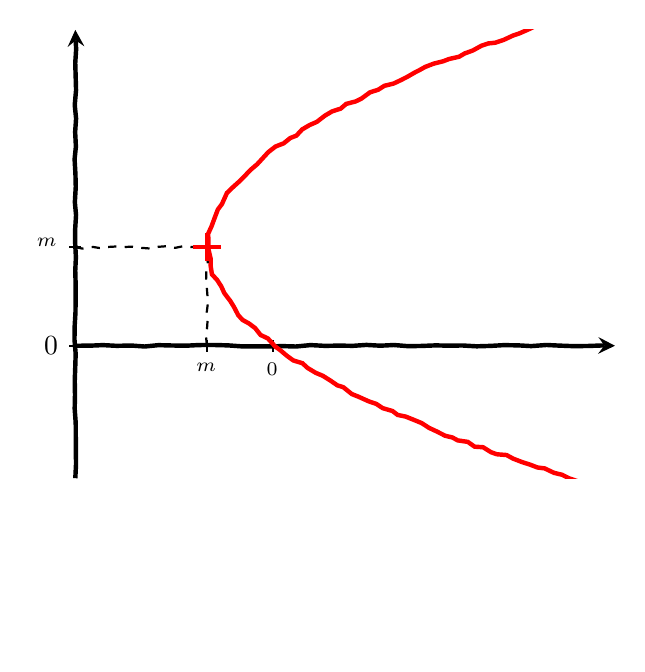
\begin{tikzpicture}%[decoration={random steps, segment length=1mm, amplitude=0.2pt}]
  \def\cxz{1.5}
  \def\KK{0.5}
  \def\czm{1.0}
  \def\cza{3.0}
  \def\cxm{1.0}
  \begin{axis}[%
      style = {ultra thick, black},
      axis x line = middle,
      axis y line = left,
      xlabel = {\cd},
      ylabel = {\cl},
      y label style = {at={(-0.05,0.95)},rotate=-90},
      xtick = {\cxm,\cxz},
      xticklabels = {$\Cd^m$,$\Cd^0$},
      ytick = {0,\czm},
      yticklabels = {0,$\Cl^m$},
      xmin = 0, xmax = 4.1,
      % ymax = 4.1,
      decoration={random steps,segment length=5pt,amplitude=0.3pt},%decorate,
      every tick/.style={thick,black,decorate}
    ]
    \begin{scope}[decoration={random steps,segment length=3pt,amplitude=0.5pt},decorate]
      \addplot[ultra thick,red,domain = -1:3,samples=30,samples y=0] ({\cxz+\KK*(\cza*x)*((\cza*x)-2*\czm)},{\cza*x});
      % \addplot[only marks] coordinates ({\cxm},{\czm});
      % \node[mark=+] (axis cs: \cxm,\czm){};
      \draw[dashed,thick, black, decorate] (axis cs: 0,\czm) -- (axis cs: \cxm,\czm);
      \draw[dashed,thick, black, decorate] (axis cs: \cxm,0) -- (axis cs: \cxm,\czm);
    \end{scope}
    \addplot [ultra thick, red, mark=+, mark size=5, mark options={solid}, only marks, forget plot]
    coordinates{(\cxm,\czm)};
  \end{axis}

\end{tikzpicture}
    \caption{Schéma présentant les coefficients d'une polaire aérodynamique.}
    \label{fig:schemas-polaire}
\end{figure}

\subsection{Pareto-optimalité}
\begin{table}
    {
    \footnotesize
    \pgfplotstabletypeset[
        columns={weights,CD,CL,fRCS,avg RCS,SREF,N cycle},
        col sep=comma,
        fixed,precision=1,
        columns/weights/.style={column name={$w$},column type = >{\centering}m{\widthof{baseline}}|,string type},
        columns/CD/.style={column name={\cd},column type={S[round-mode=places, round-precision=2, scientific-notation=engineering, table-format=4.2e+1, exponent-product = \cdot]},
        string type},
        columns/CL/.style={column name={\cl},column type={S[round-mode=places, round-precision=1, scientific-notation=engineering, table-format=4.1e+1, exponent-product = \cdot]},
        string type},
        columns/fRCS/.style={column name={$F_{RCS}$},column type={S[round-mode=places, round-precision=2, scientific-notation=engineering, table-format=5.2e+1, exponent-product = \cdot]},
        string type},
        columns/avg RCS/.style={column name={$\hat\sigma$},column type={S[round-mode=places, round-precision=1, scientific-notation=engineering, table-format=3.1e+1, exponent-product = \cdot]},
        string type},
        columns/SREF/.style={column name={\sref},numeric type},
        columns/N cycle/.style={precision=0,numeric type},
    ]
    {tables/Paretto2.txt}
\pgfplotstabletypeset[
        columns={weights,CD,CL,fRCS,avg RCS,SREF,N cycle},
        col sep=comma,
        fixed,precision=1,
        columns/weights/.style={column name={$w$},column type = >{\centering}m{\widthof{baseline}}|,string type},
        columns/CD/.style={column name={\cd},column type={S[round-mode=places, round-precision=2, scientific-notation=engineering, table-format=4.2e+1, exponent-product = \cdot]},
        string type},
        columns/CL/.style={column name={\cl},column type={S[round-mode=places, round-precision=1, scientific-notation=engineering, table-format=4.1e+1, exponent-product = \cdot]},
        string type},
        columns/fRCS/.style={column name={$F_{RCS}$},column type={S[round-mode=places, round-precision=2, scientific-notation=engineering, table-format=5.2e+1, exponent-product = \cdot]},
            string type},
        columns/avg RCS/.style={column name={$\hat\sigma$},column type={>{\centering}S[round-mode=places, round-precision=1, scientific-notation=engineering, table-format=3.1e+1, exponent-product = \cdot]},
        string type},
        columns/SREF/.style={column name={\sref},numeric type},
        columns/N cycle/.style={string type},
    ]
    {tables/baseline.txt}
    }
    \caption{Résumé des valeurs des critères et des contraintes pour certains points du front de Pareto.}
    \label{tab:recap}
\end{table}

\lipsum

\begin{figure}[htp]
    \centering
    \begin{tikzpicture}
    \begin{axis}[
        xlabel={\cd},
        ylabel={$F_{RCS}$},
        legend pos=north east,
        legend entries = {Pareto front, baseline},
    ]
        \addplot[mark=o,point meta=explicit symbolic,nodes near  coords*] table [x=CD,y=fRCS,meta=weights,col sep=comma] {tables/Paretto2.txt};
        \addplot[only marks,color=orange] table [x=CD,y=fRCS, meta=weights,col sep=comma] {tables/baseline.txt};
    \end{axis}
\end{tikzpicture}

    \caption{Front de Pareto}
    \label{fig:pareto-front}
\end{figure}

